\chapter*{Введение}
\label{ch:intro}
\addcontentsline{toc}{chapter}{Введение}

\newthought{Эта книга} предназначена для школьников и студентов. 
Вы познакомитесь с работой базы Викиданных и языком запросов SPARQL, 
с помощью которого можно работать с этой базой. 
Прочитав книгу, вы сможете извлекать из Викиданных информацию с~помощью SPARQL-скриптов, 
затем обрабатывать её и строить по ней таблицы, графики и карты.

\newthought{Цель} этой книги быть учебником по Викиданным и языку SPARQL.

\vspace{4mm}

Викиданные~--- это искусно сделанная база данных, которая как огромный кит лежит в основе громадной планеты Википедии\marginnote{%
%
Подробнее о Викиданных читайте главу <<\nameref{ch:ReviewAboutWD}>> на с.~\pageref{ch:ReviewAboutWD}
%
}. 
Впечатляет скорость роста этого кита, во многих главах мы будем обращать на это внимание.
Если изначально Викиданные создавались для обслуживания нужд Википедии, 
то сейчас Викиданные используются крайне широко и в самых разных целях.

\newthought{Опишем} структуру книги. 

\newthought{В первой части книги}\marginnote{%
%
Часть <<\nameref{part:foundation}>> на с.~\pageref{part:foundation}
%
} описано, 
что такое листинги программ, как ими пользоваться, даны базовые понятия об объектах Викиданных. 
Большая глава <<Обзор Викиданных>> включает историческую справку, 
вопрос качества данных и связи с Википедией. 
Описан сервис WDQS, к которому мы будем обращаться на каждой странице. 
Также включён небольшой обзор научных исследований, связанных с Викиданными. 
Глава <<Корзины и мячи>> с помощью образов и аналогий позволяет подступиться к Викиданным тем, 
кто хочет научиться программировать. 

%включает в себя 10 уроков, описывающих язык программирования и протокол SPARQL.
%\newthought{Вторая часть} содержит рецепты решения самых разных практических задач, 
%возникающих при работе с объектами Викиданных.

\newthought{Во второй и основной части}\marginnote{%
%
Часть <<\nameref{part:research}>> на с.~\pageref{part:research}
%
} 
каждая глава~--- это небольшое приключение, 
где один из объектов Викиданных является главным героем. 
С помощью SPARQL-запросов мы пытаемся расспросить Викиданные об этом герое, 
с помощью графиков, таблиц, диаграмм проанализировать и нарисовать себе его образ. 


\newthought{В третьей части}\marginnote{%
%
Часть <<\nameref{part:advanced}>> на с.~\pageref{part:advanced}
%
} % 
рассмотрен вопрос защиты страниц в вики-проектах, 
рассказано о сервисе балансировки ProWD 
 и то, как можно последовательно двигаться от SPARQL-запросов 
к языку Python при создании компьютерных программ (ботов), редактирующих Викиданные. 


\newthought{Заключительный раздел}\marginnote{%
%
Часть <<\nameref{part:conclusion}>> на с.~\pageref{part:conclusion}
%
} % 
собрал ответы на вопросы, рассеянные по всей книге. 
В конце книги приведён список литературы 
и индекс ключевых слов для удобного постраничного поиска.

\newthought{В исследованиях} объектов Викиданных приняли участие студенты ПетрГУ в рамках курса <<Программирование Викиданных>>, 
представленного на сайте Викиверситет\marginnote{%
Курс 
\href{https://ru.wikiversity.org/?curid=23388}{https://ru.wikiversity.org/wiki/Программирование\_Викиданных}
}. 
Этот курс растёт и пишется вместе с этой книгой. 

Потребовалось несколько лет работы со студентами в Википедии, прежде чем мы пришли с ними к таким проектам, 
как Викиверситет и Викиданные. 
Результатом предыдущей работы в Википедии стало учебное пособие для тех, 
кто хочет научиться редактировать мировую энциклопедию\autocite{Krizhanovsky2015}.

% \newthought{Книга научит} вас делать ... todo
%\vspace{5mm}


\newthought{Будет ли в этой книге рассказано}, 
как редактировать и пополнять Викиданные новой информацией? 

Нет, хотя это не сложнее, чем писать текст в SMS 
или статью в Википедии. В этом учебнике мы покажем вам, 
как увлекательно формулировать вопросы на языке Викиданных. 


\newthought{Почему мы занялись и увлеклись Викиданными?}

Потому что это самая большая, сложная 
и быстрорастушая база данных на Земле. 
Потому что эта база лежит в основе Википедии, которую может редактировать каждый.
И Викиданные тоже может редактировать каждый. 
Часто редакторы родственных проектов (Википедии, Викисклада, Викисловаря) 
заглядывают в Викиданные, чтобы там что-то поправить, изменить. 
Работу серверов Википедии и Викиданных обеспечивают сотрудники организации Викимедиа. 



\newthought{Почему школьники?} 

Потому что вообще программирование и программирование Викиданных в частности~--- это 
увлекательная и, если увлечься, простая вещь. 
Если с помощью учителя или самостоятельно школьник увлечётся, 
то сможет программировать Викиданные, писать статьи Википедии. 
Многие школьники плодотворно работают в Википедии. 
Надеемся, что благодаря этой книге одним из первых компьютерных языков, 
изучаемых в~школе, станет язык Викиданных.

\begin{marginfigure}[0.0cm]
{
\setlength{\fboxsep}{0pt}%
\setlength{\fboxrule}{1pt}%
\fcolorbox{gray}{gray}{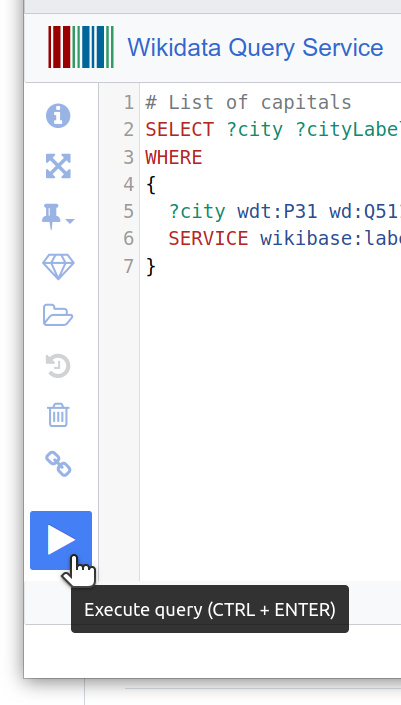
\includegraphics[width=0.65\linewidth]{./intro/WDQS_play_button.png}}
}
\caption[Выполнение скрипта в сервисе Wikidata Query Service.]{Кнопка ``Play'' запуска скрипта в сервисе Wikidata Query Service. Также скрипт можно выполнить при одновременном нажатии кнопок ``Ctrl'' и ``Enter'' на клавиатуре.}%
\label{fig:WDQS_play_button}%
\end{marginfigure}%
Покажем прямо сейчас, что Викиданные находятся от нас на расстоянии одного клика.
Откройте на компьютере или на телефоне такую ссылку: 
\url{https://w.wiki/4cXU}. 
Вы увидите главное окно, в котором мы с вами будем писать наши небольшие програмы. 
Если вы нажмёте большую синюю кнопку с белым треугольником (рис.~\ref{fig:WDQS_play_button}), 
то запустите эту программу из семи строк. 
Программа обратится к базе данных 
и спросит, какие столицы есть в Викиданных?
Результатом будет список столиц\sidenote[][1\baselineskip]{%
%
Подробнее о городах в Викиданных читайте в главе <<\nameref{ch:city}>> на с.~\pageref{ch:city}. 
}. % 

Вот так просто можно запускать программы в этой книге: достаточно браузера, 
Интернета и гиперссылки с запросом к Викиданным.



